\documentclass{beamer}
\usetheme{Hannover}
\setbeamersize{sidebar width left=0pt}
\usepackage[T1, T2A]{fontenc}
\usepackage[utf8]{inputenc}
\usepackage[russian]{babel}
\usepackage{hyperref}
\usepackage{graphicx}
\graphicspath{ {../Images/} }

\author{Григорий Матюхин}
\date{\today}
\title{Лабораторная работа \textnumero4.}
\subtitle{Работа с программными пакетами}

\begin{document}
\begin{frame}[plain]
	\titlepage
\end{frame}
\section{Цель работы}
\begin{frame}[plain]
	\frametitle{Цель работы}
	Получить навыки работы с репозиториями и менеджерами пакетов.
\end{frame}

\section{Последовательность выполнения работы}
\subsection{Работа с репозиториями}
\begin{enumerate}
	\begin{frame}[plain]
		\item В консоли перейдите в режим работы суперпользователя.
		\item Перейдите в каталог \texttt{/etc/yum.repos.d} и изучите содержание каталога и файлов репозиториев:
		\\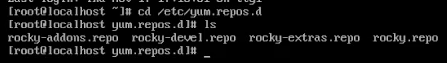
\includegraphics{1.png}
		\item Выведите на экран список репозиториев и поясните полученную информацию.
		\\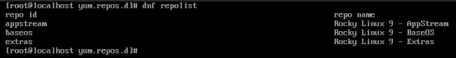
\includegraphics{2.png}
	\end{frame}
	\begin{frame}[plain]
		\item Установите \texttt{nmap}, предварительно изучив информацию по имеющимся пакетам.
		\\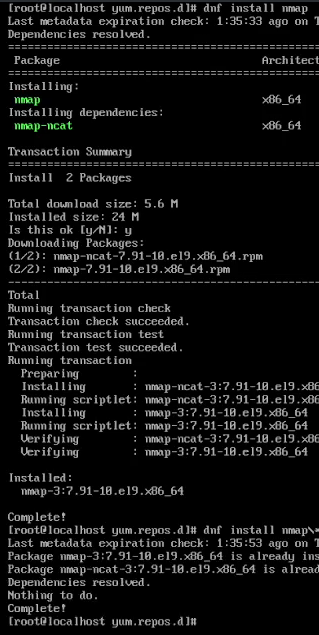
\includegraphics{3.png}
	\end{frame}
	\begin{frame}[plain]
		\item Удалите \texttt{nmap}:
		\\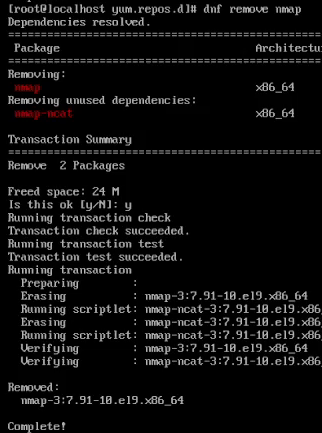
\includegraphics{4.png}
	\end{frame}
	\begin{frame}[plain]
		\item Установите группу пакетов \texttt{RPM Development Tools}:
		\\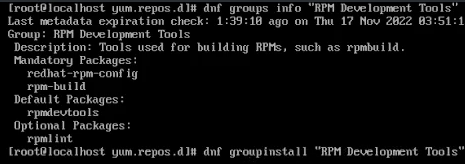
\includegraphics{5.png}
	\end{frame}
	\begin{frame}[plain]
		\item Посмотрите историю использования команды \texttt{dnf} и отмените последнее, например шестое по счёту, действие:
		\\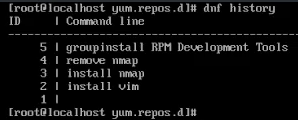
\includegraphics{6.png}
	\end{frame}

\end{enumerate}

\subsection{Использование rpm}
\begin{frame}[plain]
	\frametitle{Использование rpm}
	Предположим, что требуется установить текстовый браузер \texttt{lynx} из rpm-пакета
\end{frame}
\begin{enumerate}
	\begin{frame}[plain]
		\item Скачайте rpm-пакет \texttt{lynx}:
		\item Найдите каталог, в который был помещён пакет после загрузки:
		\item Перейдите в этот каталог и затем установите rpm-пакет:
	\end{frame}
	\begin{frame}[plain]
		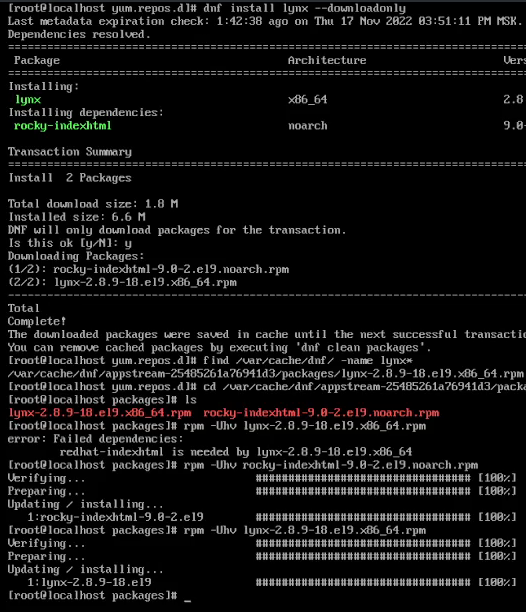
\includegraphics{7.png}
	\end{frame}
	\begin{frame}[plain]
		\item Определите расположение исполняемого файла:
		\item Используя \texttt{rpm}, определите по имени файла, к какому пакету принадлежит \texttt{lynx} и получите дополнительную информацию о содержимом пакета:
		\\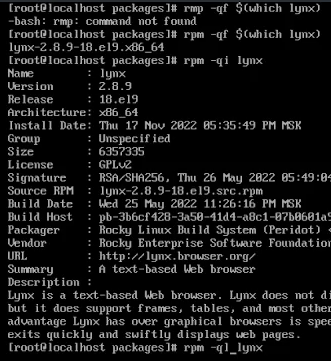
\includegraphics{8.png}
		\item Получите список всех файлов в пакете, используя, а также выведите перечень файлов с документацией пакета, посмотрите файлы документации, применив команду \texttt{man lynx}.
	\end{frame}
	\begin{frame}[plain]
		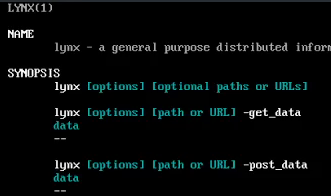
\includegraphics{9.png}
	\end{frame}
	\begin{frame}[plain]
		\item Выведите на экран перечень и месторасположение конфигурационных файлов пакета:
		\item Выведите на экран расположение и содержание скриптов, выполняемых при установке пакета и поясните, для чего предназначены скрипты, если они есть.
		\\
\includegraphics{10.png}
		\item В отдельном терминале под своей учётной записью запустите текстовый браузер \texttt{lynx}, чтобы проверить корректность установки пакета.
		\\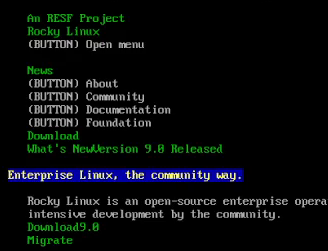
\includegraphics{11.png}
	\end{frame}
	\begin{frame}[plain]
		\item Вернитесь в терминал с учётной записью \texttt{root} и удалите пакет:
		\\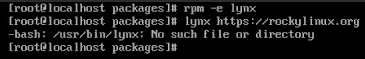
\includegraphics{12.png}
	\end{frame}
\end{enumerate}

\begin{frame}[plain]
	Предположим, что требуется из rpm-пакетов установить \texttt{dnsmasq}\\ (DNS-, DHCP- и TFTP-сервер).
\end{frame}
\begin{enumerate}
	\begin{frame}[plain]
		\item Установите пакет \texttt{dnsmasq} и определите расположение исполняемого файла:
		\item Определите по имени файла, к какому пакету принадлежит \texttt{dnsmasq} и получите дополнительную информацию о содержимом пакета:
		\item Получите список всех файлов в пакете, а также выведите перечень файлов с документацией пакета, посмотрите файлы документации, применив команду \texttt{man dnsmasq}.
		\\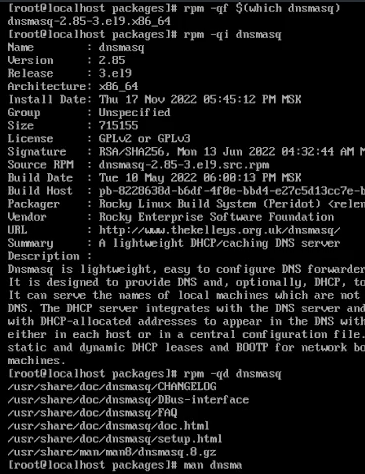
\includegraphics{13.png}
	\end{frame}
	\begin{frame}[plain]
		\item Выведите на экран перечень и месторасположение конфигурационных файлов пакета:
		\item Выведите на экран расположение и содержание скриптов, выполняемых при установке пакета и поясните, для чего предназначены скрипты.
		\\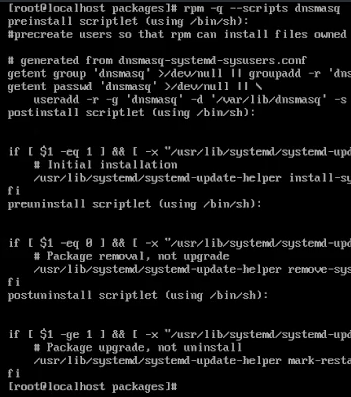
\includegraphics{14.png}
	\end{frame}
	\begin{frame}[plain]
		\item Вернитесь в терминал с учётной записью \texttt{root} и удалите пакет:
		\\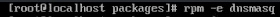
\includegraphics{15.png}
	\end{frame}
\end{enumerate}

\section{Вывод}
\begin{frame}[plain]
	\frametitle{Вывод}
	В ходе выполнения данной работы я получил навыки работы с репозиториями и менеджерами пакетов.
\end{frame}

\end{document}
